 \documentclass[12pt]{article}
\usepackage{geometry}
\usepackage{gensymb}
\usepackage[utf8]{inputenc}
\usepackage{tcolorbox}
\usepackage{multicol}
\usepackage{enumitem}
\usepackage{fancyhdr}
\usepackage{indentfirst}
\usepackage[bf,center]{titlesec}
\usepackage{tocloft}
\usepackage{hyperref}
\usepackage{tabularx}
\usepackage{ragged2e}
\usepackage{tocloft}
\usepackage{secdot}
\usepackage[T1]{fontenc}

\hypersetup{
	colorlinks=true,
	linkcolor=black,  
	urlcolor=blue
}

\urlstyle{rm}

\titlespacing*{\section}{3pt}{3pt}{5.5pt}
\titlespacing*{\subsection}{0pt}{1.5\baselineskip}{2.5pt}
\titlespacing*{\subsubsection}{0pt}{0.5\baselineskip}{1.5pt}
\titleformat{\section}{\large \bfseries \centering}{\thesection.}{1em}{}
\titleformat{\subsection}{\normalsize \bfseries
	\centering}{\thesubsection.}{1em}{}
\titleformat{\subsubsection}{\normalsize \bfseries
	\centering}{\thesubsubsection.}{1em}{}
\geometry{b5paper, left=2cm, right=2cm, top=2.5cm, bottom=2.5cm}
\pagestyle{fancy}
\fancyhead{}
\fancyfoot{}
\fancyfoot[R]{\thepage}
\renewcommand{\headrulewidth}{0pt}
\linespread{1}
\setlength{\parindent}{1cm}
\setlength{\parskip}{0pt}
\renewcommand{\contentsname}{\hspace*{\fill}\bfseries\large Sadržaj\hspace*{\fill}} 
\renewcommand{\cfttoctitlefont}{\centering\bfseries\large}
\renewcommand{\cftsecfont}{}
\renewcommand{\cftsecpagefont}{}
\renewcommand{\cftsecleader}{\cftdotfill{\cftsecdotsep}}
\renewcommand\cftsecdotsep{\cftdot}
\renewcommand\cftsubsecdotsep{\cftdot}
\renewcommand{\cftsecaftersnum}{.}
\renewcommand{\cftsubsecaftersnum}{.}
\AddToHook{cmd/section/before}{\clearpage}

\renewcommand{\figurename}{Slika}

\begin{document}
	
	\begin{titlepage}
		\thispagestyle{empty}
		\begin{center}
			\vspace*{1cm}
			\begin{large}\textbf{Univerzitet u Beogradu}
				
				\textbf{Matematički fakultet}
				
				\vspace{4cm}
				\textbf{\huge{Informacione tehnologije kroz evoluciju društva}}
			\end{large}
			
		\end{center}
		\vspace{7cm}
		\begin{flushright}
			Autor: \textbf{Predrag Mitić}
			

		\end{flushright}
		\vspace{1cm}
		\begin{center}
			Beograd, Decembar 2022
		\end{center}
	\end{titlepage}
	
	\tableofcontents
	
	\pagebreak
	
	\section{Uvod}
	
	Nastanak računara vezan je za vekovnu težnju čoveka da sebi olakša proces računanja, ubrza ga i učini tačnijim. Ideja o konstruisanju uređaja za automatizaciju izračunavanja stara je nekoliko hiljada godina. Prva naprava te vrste je abakus (abacus). Abakus je prva poznata sprava za računanje starih Grka, Egipćana, Kineza i Rimljana. Abakus je najčešće napravljen od drveta. Sastoji se od okvira sa kuglicama ili kamenčićima koji su nabodeni na štapiće ili žicu, ili se kuglice povlače po izrezbarenim otvorima. Kuglice ili kamenčići svojim položajem predstavljaju vrednost određenog broja. Abakus omogućava i rešavanje malo komplikovanijih računskih operacija. Pored osnovnih računskih operacija (sabiranja, oduzimanja, množenja i deljenja) na njemu je moguće i korenovanje.
	
	Tehnološki razvoj, posebno elektronskih računara, izazvao je najkorenitije i najbrže promene u svakodnevnom načinu života ljudi. Razna otkrića i inovacije iz oblasti računarskih tehnologija imaju veliki uticaj, koji pored sopstvenog razvoja pojedinca, doprinose razvoju svih grana ljudske delatnosti koje baš i nisu imale pozitivan odziv na nove  i brze mogućnosti za napredovanje. Međutim, digitalna baza podataka, kao i njihova numerička, tekstualna i grafička obrada, predstavili su uvod u najveći pojedinačni iskorak u računarskoj istoriji, a to su računarske mreže.
	
	Društvo se zasniva na komunikaciji. Što bi značilo da je čovečanstvo počelo da se razvije kad su ljudi polčeli da govore. Evolucija se polako odvija i nijedna velika promena nije došla preko noći. Za ovaj rad nije neophodno davati detaljna razvoj evolucije pa ćemo isti i preskočiti. 
	
	Održivo očekivanja omogućavaju da ove komunikacije imaju mesto u svakodnevnom životu ljudi i čine mogućim novi načini organizovanja za povezivanje među njima i odnos prema ostatku sveta. Ova teorija podrazumeva da je definisanje evolucije kao niza etapa pomalo veštački. Iz tog razloga, moramo pretpostavitiv da su ove teorije od vitalnog značaja za identifikaciju ključnih momenata u evolucije ljudskog društva.
	
	Proces evolucije se veoma ubrzao, ljudi su počeli da razmišljaju o globalnom društvo.  Aleksandrova, a kasnije i Rimska osvajačka ambicija zahvatio ceo svet. Razum se probudio, a nauka razvijala.  Znanje je postalo samo po sebi cilj, i nepoznato se svuda istraživalo, da li kroz otkrivanje zakona univerzuma ili otkrivanje misterija tela i uma.
    
    \section{Istorija razvoj komunikacionih tehnologija}
    
    Pre pet stotina godina, tačnije 1450. g, izmišljena je štamparska mašina i time je započeta nova era na polju komunikacije. Prvi put je moglo da se masovno proizvodi literatura i da se znanje širi i ostavlja budućim generacijama. Štamparska presa je napravila revoluciju u komunikaciji. Sada su knjige bile dostupne širokim masama što nije bio slučaj sa ručno pisanim knjigama. Pošto su se knjige ranije prepisivale ručno, često je dolzilo do grešaka i gubile su se neke važne misli autora. Kod štampanih knjiga se to nije dešavalo jer su bile kopije originala ili najstarih dostupnih prepisa. Tako smo sada imali nove kopije koje su bile bolje od starih, rukom pisanih. To je važno jer je društvo pre toga uvek davalo prednost starim stvarima u odnosu na nove, a ovo je bila prva inovacija koja je dala prednost novitetima i moderno je postajalo vrednije od starog.
    
\begin{figure}
    \centering
    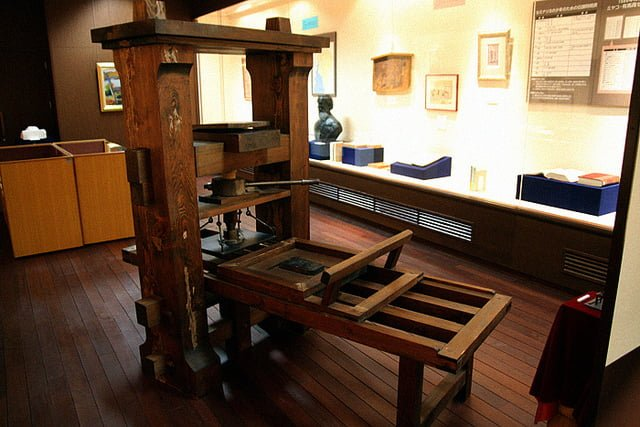
\includegraphics[scale=0.4]{stamparska-presa.jpg}
    \caption{Štamparska presa}
\end{figure}


	Samoobrazovanje je postalo moguće, postignut je veliki napredak u sticanju znaja o svetu, čoveku, prirodi i društvu. Filozofska misao je bila zaštićena od zaborava u mnogo većoj meri i mnogo lakše se širila. Zbog toga smo imali popularizaciju demokratije kao oblika vladavine umesto monarhije koja je bila opšte prihvaćena do tada. Ustavima je uspostavljena veza između pravnog i političkog sistema, što je donelo vladavinu prava. Ubrzo su ljudska prava prihvaćena širom sveta, u kojem su do skora tortoru i javna pogubbljenja bila svakodnevnica. 
	
	Štampanje je umnogome olakšalo protok informacija i znanja. Vesti su se mnogo brže širile izvan lokalnog konteksta preko novina i raznih časopisa. Time se je proširilo interesovanje ljudi o svetskim događajima i novim idejama za napredak.

	To doba nzivamo mehaničkim dobom, odnosno dobom kada su mehaničke mašine uzrokovale evoluciju čovečanstva.

	Sledeći važan korak je usledi četiri veka nakon štamparske mašine i to je bio telegraf, kasnije su se promene u komunikaciji dešavale mnog češće. Ovo je bio period kada je došlo do naglog razvoja telekomunikacija i elektromehaničkog izračunavanja. Otkriće načina iskorišćavanja elektriciteta za potrebe izračunavanja je predstavlja ključ napretka na ovim poljima. Elektricitet se vemo brzo prenosi na velike udaljenosti pa smo time dobili veliki protok invformacija u, do tada, ne zamislivo kratkom vremenu.
	
	Par decenija nakon telegrafa izmisljen je telefon, odnosno radio, koji  su bili osnova za sve savremene telekomunikacione izume. Svi ti izumi došli su na ovaj svet iz ljudkse potrebe za komunikacijom, bržom i lakšom komunikacijom ljudi koji su na velikoj u daljenosti, bez mogućnosti razgovora licem u lice. 

	
\begin{figure}
    \centering
    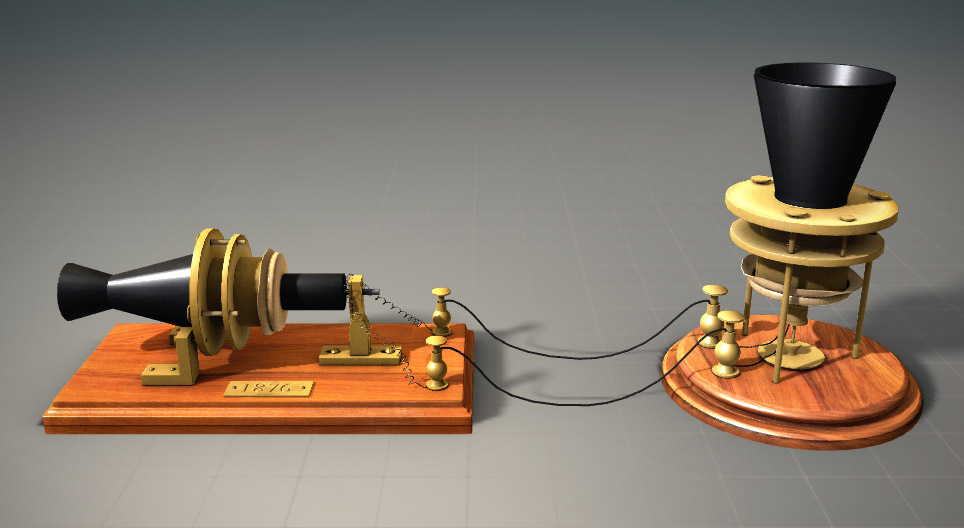
\includegraphics[scale=0.4]{telefon.jpg}
    \caption{Belov telefon}
\end{figure}

	Elektronika, kako sama, tako i na polju informacionih tehnologija doživljava vrtoglavi napredak. U prvoj polovini XX veku je zabeležen izum televizije, što je bio prvi put da se video sadršaj prenosi širokom auditorijumu. To je bio još jedan korak prema današnjem načinu komunikacije, o kome ćemo malo kasnije više reći.
	
	Poznavanjem elektronike i elktromagnetnih talasa, brzo se došlo na ideju bežične komunikacije. Lansiranjem prvih satelita u orbitu napravljen je veliki napredak i na tom polju. Sateliti su imali zadatak da primaju signal sa stanica na zemlji, pojačavaju ga i prosleđuju ka drugim stanicama koje su hiljadama kilometara daleko. 
	
	Mobilni telefon je sledeća prekretnica u komunikacionom pogledu. Ljudi više ne moraju da imaju elektronsku vezu između sebe da bi razgovarali na većim udaljenostima, već je bilo dovoljno da imaju mobilni telefon koji komunicira sa drugim mobilnim telefonom preko repetitora, sto je slično satelitskoj komunikaciji, samo što su repetitori na zemlji. 
	
	U tom periodou je pronađen i internet, koji je uključio i računare u komunikaciju. Pre interneta sa postojale neke lokalne mreže koje su omogućavale komunikaciju između umreženih računara, ali to nije bilo globalno upotrebljivo. Sa internetom dobijamo mogućnost da, povezivanjem na tu mrežu, možemo da stupimo kontakt sa svim ostalim računarima na svetu, narvno koji su nakačeni na mrežu. Ovo je bilo jedan od najvećih napredaka u komunikaciji koji je omugućio, u početku brzu razmenu dokumenata, poruka i sličnog, a kasnije poziva, video poziva kao i javnog iznosenja misljnja preko društvenih mreža i mnogo druge pogodnsti koje ranije nisu bile zamislive.

   
    \section{Savremeno društvo i komunikacija}
    
    
	Danas tehnologija menja pejzaž sveta i vodi nas ka sofisticiranom tehničkom svetu koji je sve više na usluzi običnom čoveku. Od nastanka čovečanstva komunikacija je, dakle, bila ustavna osnova društva.
	
	Evolucija ljudskog društva ubrzala je svoj ritam. Ono što u stvarnosti nije postojalo može se zamisliti i komunicirati kako bi se pronašlo i uradilo. Polazeći od osnovnih postulata uspešnosti poslovanja, neosporno se ustanovljava da je ključ uspeha rezultat kontinuiranog obavljanja niza temeljno razmotrenih aktivnosti usmerenih na sistematično planiranje i neprekidno usklađivanje poslovanja sa kompleksnim i promenljivim okruženjem. 
	
	Savremeni uslovi privređivanja generisani su neprestanim razvojem talasa razornih inovacija i neumitno dovode do neophodnosti adekvatnog prilagođavanja i redefinisanja poslovanja kroz povećanje stepena integracije inovativnih tehnologija u njegove postojeće tokove bez disrupcije posojećeg.
	
	Ovi iterativno-inkrementalni talasi inovacija, praćeni upotrebom novih digitalnih tehnologija, omogućavaju i utiču na stvaranje novih poslovnih modela kao svojevrsnih nosioca transofrmacionih promena. 
	
	Pored potencijala za revolucionarna unapređenja poslovanja, razvoj informaciono-komunikacionih tehnologija dovodi i do pitanja problema njihove optimalne operacionalizacije u smislu nemogućnosti potpune implementacije adekvatne zaštite digitalnog nastupa od pretnji i rizika koje ove disruptnivne inovacije i tehnologije generišu.
	
	Kao što smo već rekli u ovom radu, savremoeno društvo jeste konačni proizvod duboke transformacije društva izvedenog iz otkrića štamparske mašine. Preko novina koje su omogućavale širenje vesti na dnevnom nivo. Sada imam elektronski oblik novina i vesti se šire za manje od jednog minuta na nivo celog sveta.  Za tu pojavu je kriv internet (Slika 3). 


\begin{figure}
    \centering
    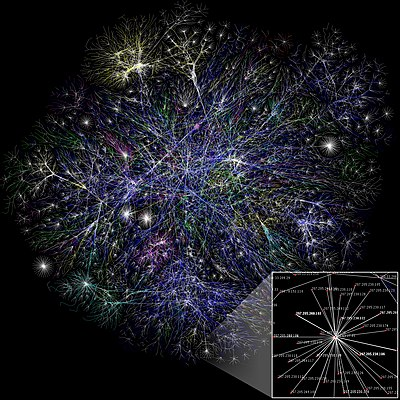
\includegraphics[scale=0.4]{internet.jpg}
    \caption{Veličina interneta}
\end{figure}
	

	Internet nam je dao neke nove načine za komunikaciju i time potpuno promenio pogled na svet. U nastavku ću vam reći malo više o tome kako izgleda moderni svet sa internetom u pogledu komunikacije.
	
	Elektronska pošta je jedan od njih. Sada pisma više ne putuju danima od pošiljaoca do rimaoca, već je dovoljan jedan klik i par sekundi čekanja da pismo bude dostavljenjo. Ovo je važan komunikacioni servis koji je dostupan na Internetu. Koncept slanja elektronskih tekstualnih poruka između osoba koje komuniciraju na način koji je analogan slanju pisama ili memoranduma je prethodio formiranju interneta. Elektronska posšta je jednako moćna, ili čak i moćnija od obične. Daje mogućnosti slanje dodatnih dokumenata, slika i raznih drugih fajlova. Sve je to moguće slati i na više različitih adresa ođednom.
	
	U poslednje vreme, primećujemo i da se sve češće obični telefonski razgovori zamenjuju razgovorima preko interneta, za koje je dovoljno imati internet konekciju, a sve ostalo je besplatno. Internet telefonija je široko rasprostranjena u svetu dana. To nam je omogućeno VoIP protokolom (Voice-over-Internet Protocol). Kvalitet zvuka još uvek može da varira od poziva do poziva, mada je obično jednak ili bolji od tradicionalnih poziva.
	
    Današnji pozivi preko interneta (Slika 4) daju dosta veće mogućnosti od klasičnih telefona, kao što su grupni razgovori, video pozivi, grupni video pozivi i td. Sve ovo je omogućilo neverovatne promene u savremenom svetu, što smo imali prilike da vidimo tokom Covid-19 pandemije, sve škole, kompanije i ostale ustanove su ođednom bile primorane na rad na daljinu i to im je omogućila savremena komuikaciona tehologija. Bez gotovo ikakvih posledica na produktivnost u poslu ljudi su mogli da rade od kuće i ostanu bezbedni od opakog virusa. 

    Sada često radio i televizijski distributeri pružaju internetski pristup svojim audio ili video produkcijama uživo. Oni isto tako omogućavaju odloženo gledanje ili slušanje putem raznih sistema. Sada je mnogim provajderima, koji čak i nemoju dozvul za emitovanje omogućeno da strimuju svoj sadržaj preko neke od platformi na internetu. To znači da se uređaj koji je povezan sa internetom, kao što je računar, može koristiti za pristup onlajn medijima na skoro isti način kao što je ranije bilo moguće samo sa televizorom ili radio prijemnikom. Opseg dostupnih tipova kontenta je daleko širi, od specijalizovanih tehničkih vebkasta do multimedijskih servisa koji se isporučuju po zahtevu. Podkastovanje je slično tome, ovde se obično audio materijal reprodukuje na računaru ili se prenese na neki prenosni medijski plejer i slušao u pokretu. 
    
	Jutjub koji je osnovan 15. februara 2005, je danas vodeći vebsajt za slobodni video striming sa ogromnim brojem korisnika. Taj sajt koristi flaš-bazirani veb plejer za prenos i prikazivanje video fajlova. Registrovani korisnici mogu da pošalju neograničene količine video materijala i da izgrade svoje personalne profile. Jutjub tvrdi da njihovi korisnici gledaju stotine miliona, i pošalju stotine hiljada video snimaka dnevno.

\begin{figure}
    \centering
    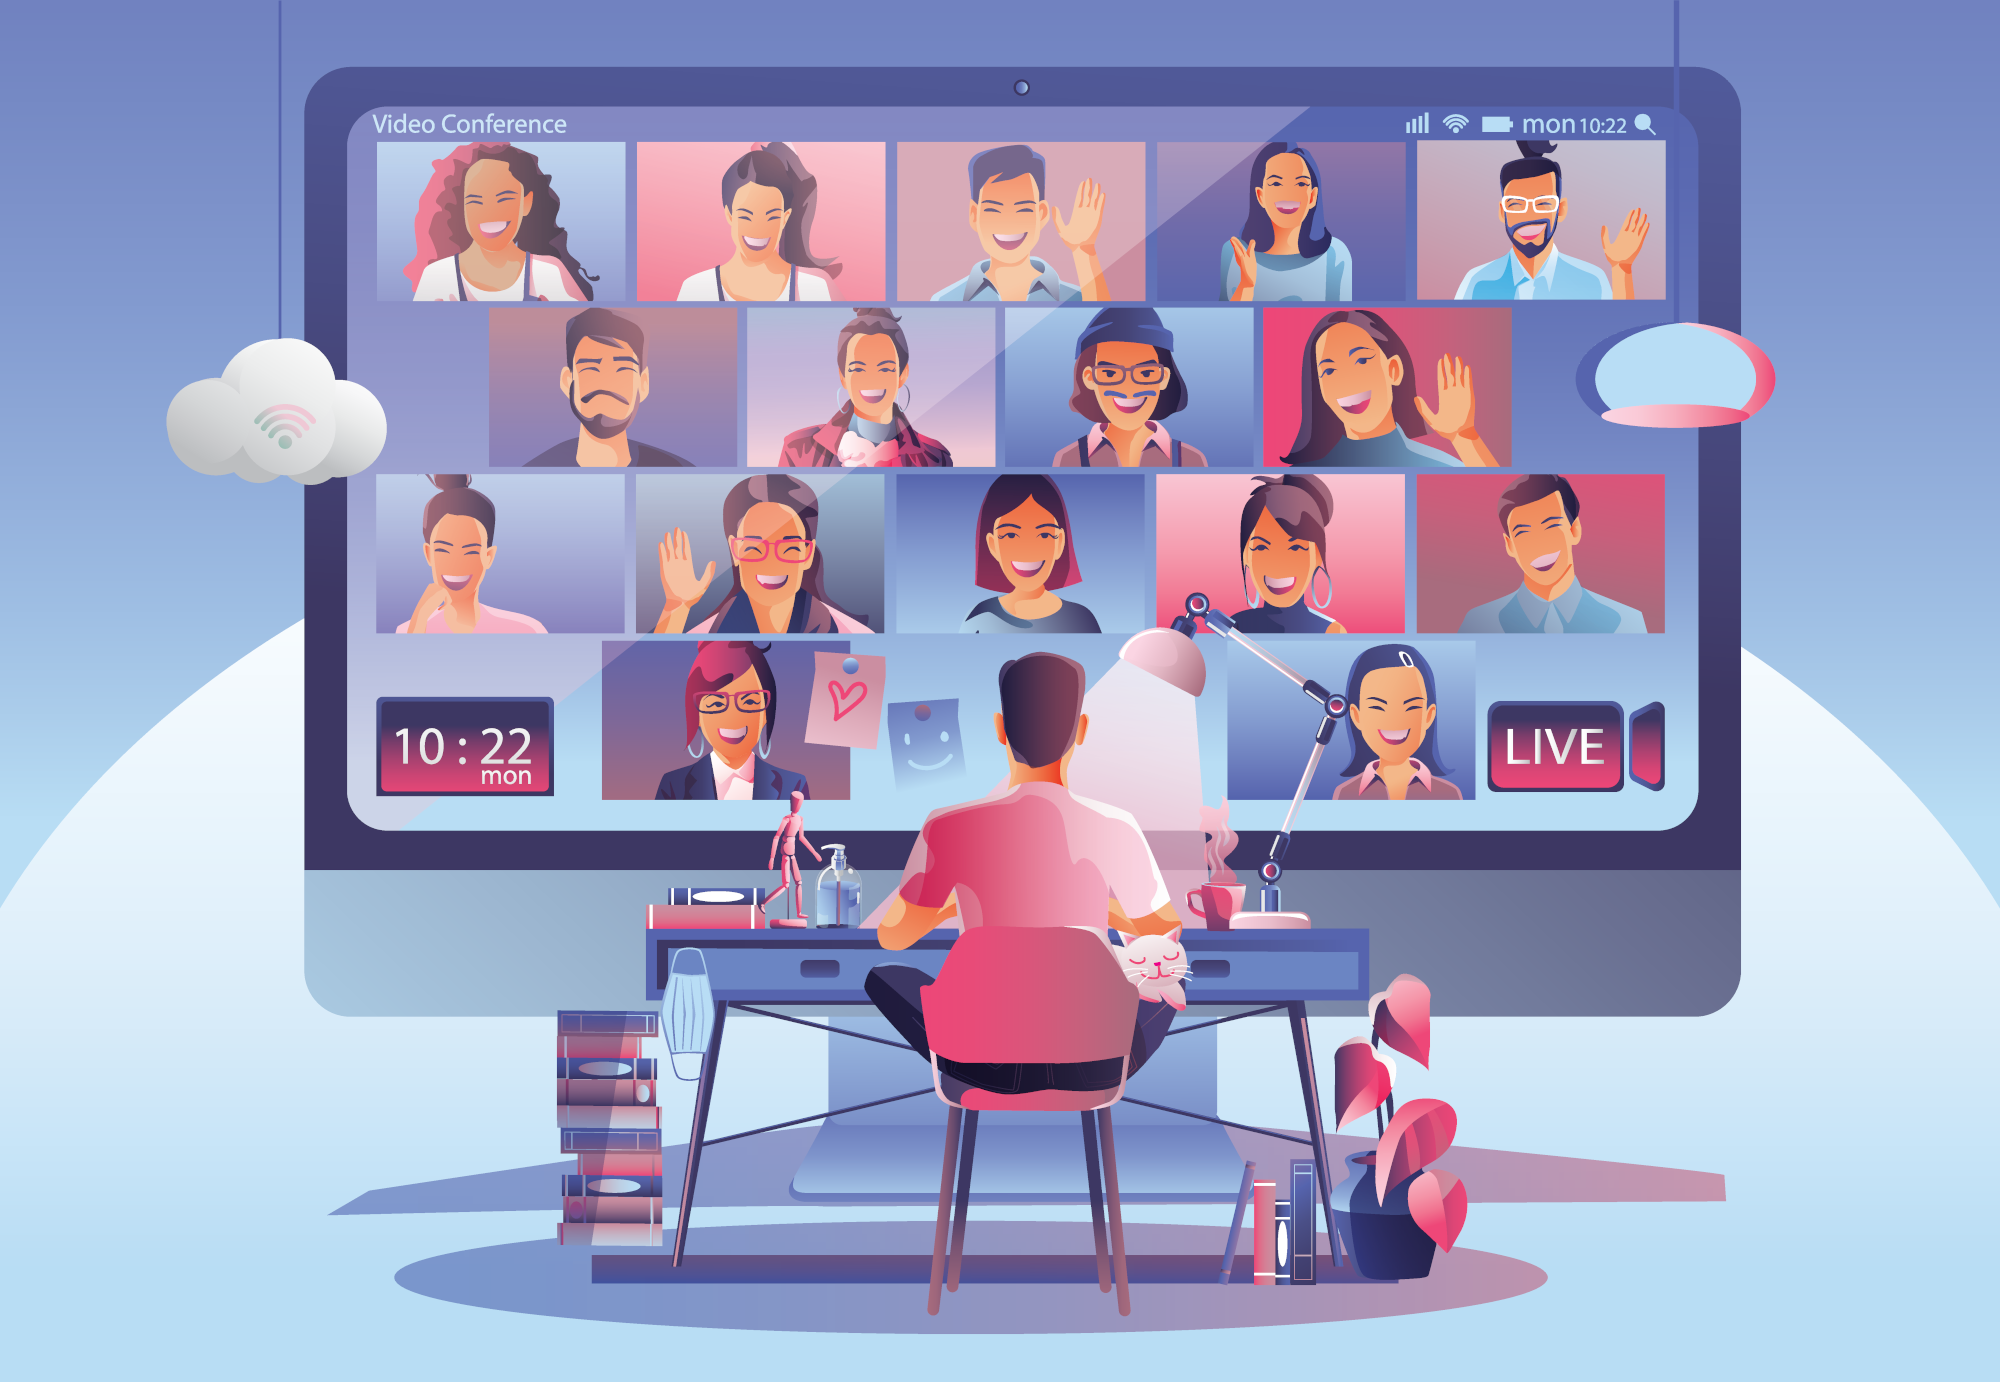
\includegraphics[scale=0.2]{poziv.png}
    \caption{Online poziv}
\end{figure}

	Savremeni načini komunikacije, ondnoso internet, nam omugućava i razmene velikih količina podataka, ako izaberemo neku drugu vrstu protokola. Računarski fajl se može poslati na vebsajt ili FTP server da bi ga drugi korisnici mogli na jednostavan način preuzeti. On se može staviti u „zajedničku lokaciju“ ili na fajl server.  Ova jednostavna svojstva interneta, na globalnoj osnovi menjaju produkciju, prodaju, i distribuciju svega što se može redukovati do računarskog fajla za transmisiju. Time su obuhvaćeni svi oblici štampanih publikacija, softverskih proizvoda, vesti, muzike, filma, videa, fotografije, grafike i drugih umetnosti. To je uzrokovalo seizmička pomeranja u svim postojećim industrijama koje su ranije kontrolisale produkciju i distribuciju tih produkata.

	Jedna od zastupljeijih servisa na internetu je internet prodaja, koja je podigla, jednu od najstarijih privrednih grana, trgovinu, na drugi nivo. Sve je manje mesta gde ljudi uživio kupuju stvari koje su im potrebne, moderni sajtovi za prodaju raznih stvari uzimaju glavno mesto u izboru za kupovinu. Od prodaje najsitnijih stvari koje vam više ne trebaju, pa sve do nekretnina, jahti, čak i kompaniji, sve se obavlja online. Za neku internet prodavnicu dovoljno je napraviti web sajt, implementirati neki sistem za plaćanje i prodaja moze da krene. Nek od najuspešnijih svetskih kompanija današnjice se upravo bave ovim poslom, kao što su Amazon, eBay, AliExpress i slične. Od 2016. godine, potrošači mogu kupovati na mreši koristeći razne računare i uređaje, uključujući desktop, laptop, tablet računare i pametne telefone.

	Pored interneta, računarske tehnologije se omogućile rzne druge olakšice čovečanstvu i time usmerile evoluciju na neku drugu stranu. U novije vreme, svedoci smo da veštačka inteligencija zauzima dosta mesta u savremenom društvu, da ne kažem preuzima posao od ljudi, ali je tako. Imamo za primer neverovatan razvoj autonomne vožnje (Slika 5) gde čovek da gotovo nije ni potreban automobilu da dođe od tačke A do tačke B, sem da ga uključi i zada mu destinaciju na koju želi da ode. Kompanija Tesla je postigla neverovatan uspeh proizvodnjom automobila sa takvom sposobnošću, pa mošemo zaključiti da su ljudi prihvatili taj savremeni način transporta. 
	
	
\begin{figure}
    \centering
    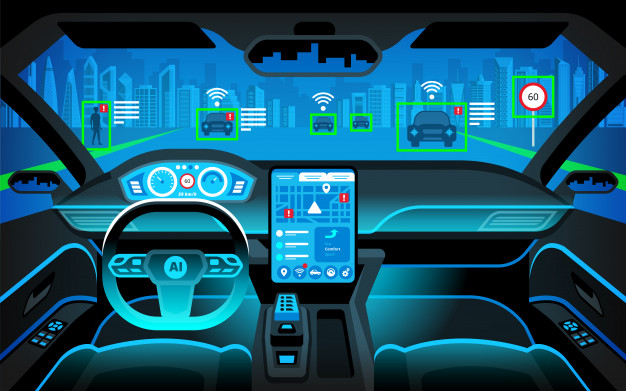
\includegraphics[scale=0.5]{car.jpg}
    \caption{Savremeni automobil}
\end{figure}
	
	Automatizacija procesa proizvodnje je takođe zanimljiva u pogledu evolucije. Današnji proizvodni pogoni su bazirani isključivo na računarima, koji gotovo sav posao obavljaju bez ljudi, uz izuzetak nekih oblasti gde su ljudi još uvek ne zamenjljivi, ali kažem još uvek, jer je samo pitanje vremena kada će računari dostići taj nivo autonomije da mogu samostalno da iznesu čitavi proizvodni proces.
    
    \section{Zaključak}
 
    Društvo se zasniva na komunikaciji. To znači da proizilazi sledeće, svaka ogromna promena koju je čovečanstvo doživelo od tehnološkog otkrića vezana je za a komunikaciju. Jezik i pismo, kao prve komunikacione tehnike, prati niz tehnologija, npr kao štamparija, telefon, radio, televizija, internet i mobilni  telefoni, koji su danas pametniji nego ikad. Ove nove tehnologije su povećale količinu komunikacija, čineći svetsko društvo složenijim nego ikad. Informaciono-komunikacione tehnologije, okarakterisanstalnim inovacijama i brzim tehnološkim promenama, jeste imajo ogroman uticaj na društvo i ubrzavo društvene promene. Međutim, evolucija ne staje.
    
    \linespread{4}
    
	\section*{Literatura}
	\subsection*{Referentni rad}
	\addcontentsline{toc}{section}{Literatura}
	
		 \item D.Rodríguez, C.Busco, R.Flores,  \emph Information technology within society's evolution, 2006
		 
	\subsection*{Pomoćni materijali}
	
		 \item Elektronska trgovina, \emph Wikipedia, https://sr.m.wikipedia.org/sr-ec/
		 \item Internet,  \emph Wikipedia,  https://sr.m.wikipedia.org/sr-ec/
		 

	
\end{document}
